\section{XMButton  Class Reference}
\label{classXMButton}\index{XMButton@{XMButton}}
{\tt \#include $<$XMPushbutton.h$>$}

Inheritance diagram for XMButton::\begin{figure}[H]
\begin{center}
\leavevmode
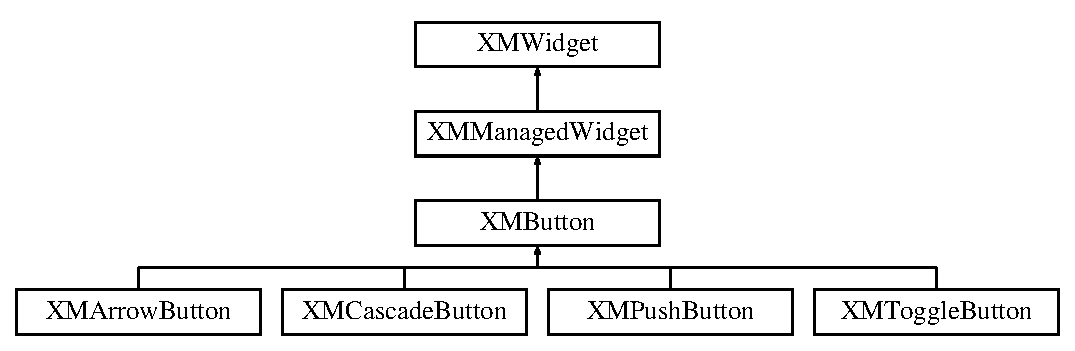
\includegraphics[height=4cm]{classXMButton}
\end{center}
\end{figure}
\subsection*{Public Methods}
\begin{CompactItemize}
\item 
virtual void {\bf Enable} ()
\item 
virtual void {\bf Disable} ()
\item 
virtual void {\bf Label} (Xm\-String label)
\item 
virtual void {\bf Label} (String label)
\item 
virtual void {\bf Set\-Mnemonic} (Key\-Sym k)
\item 
{\bf XMButton} (char $\ast$n, Widget\-Class c, Widget parent)
\item 
{\bf XMButton} (char $\ast$n, Widget\-Class c, {\bf XMWidget} \&parent)
\item 
{\bf XMButton} (Widget w)
\item 
void {\bf Set\-Accelerator} (char $\ast$translation, char $\ast$prompt)
\end{CompactItemize}


\subsection{Constructor \& Destructor Documentation}
\index{XMButton@{XMButton}!XMButton@{XMButton}}
\index{XMButton@{XMButton}!XMButton@{XMButton}}
\subsubsection{\setlength{\rightskip}{0pt plus 5cm}XMButton::XMButton (char $\ast$ {\em n}, Widget\-Class {\em c}, Widget {\em parent})\hspace{0.3cm}{\tt  [inline]}}\label{classXMButton_a5}




Definition at line 349 of file XMPushbutton.h.\index{XMButton@{XMButton}!XMButton@{XMButton}}
\index{XMButton@{XMButton}!XMButton@{XMButton}}
\subsubsection{\setlength{\rightskip}{0pt plus 5cm}XMButton::XMButton (char $\ast$ {\em n}, Widget\-Class {\em c}, {\bf XMWidget} \& {\em parent})\hspace{0.3cm}{\tt  [inline]}}\label{classXMButton_a6}




Definition at line 352 of file XMPushbutton.h.\index{XMButton@{XMButton}!XMButton@{XMButton}}
\index{XMButton@{XMButton}!XMButton@{XMButton}}
\subsubsection{\setlength{\rightskip}{0pt plus 5cm}XMButton::XMButton (Widget {\em w})\hspace{0.3cm}{\tt  [inline]}}\label{classXMButton_a7}




Definition at line 355 of file XMPushbutton.h.

\subsection{Member Function Documentation}
\index{XMButton@{XMButton}!Disable@{Disable}}
\index{Disable@{Disable}!XMButton@{XMButton}}
\subsubsection{\setlength{\rightskip}{0pt plus 5cm}virtual void XMButton::Disable ()\hspace{0.3cm}{\tt  [inline, virtual]}}\label{classXMButton_a1}




Definition at line 320 of file XMPushbutton.h.

References XMWidget::Set\-Attribute().\index{XMButton@{XMButton}!Enable@{Enable}}
\index{Enable@{Enable}!XMButton@{XMButton}}
\subsubsection{\setlength{\rightskip}{0pt plus 5cm}virtual void XMButton::Enable ()\hspace{0.3cm}{\tt  [inline, virtual]}}\label{classXMButton_a0}




Definition at line 316 of file XMPushbutton.h.

References XMWidget::Set\-Attribute().

Referenced by XMArrow\-Button::XMArrow\-Button(), XMCascade\-Button::XMCascade\-Button(), XMPush\-Button::XMPush\-Button(), and XMToggle\-Button::XMToggle\-Button().\index{XMButton@{XMButton}!Label@{Label}}
\index{Label@{Label}!XMButton@{XMButton}}
\subsubsection{\setlength{\rightskip}{0pt plus 5cm}virtual void XMButton::Label (String {\em label})\hspace{0.3cm}{\tt  [inline, virtual]}}\label{classXMButton_a3}




Reimplemented in {\bf XMArrow\-Button} {\rm (p.\,\pageref{classXMArrowButton_a9})}.

Definition at line 332 of file XMPushbutton.h.

References Label().\index{XMButton@{XMButton}!Label@{Label}}
\index{Label@{Label}!XMButton@{XMButton}}
\subsubsection{\setlength{\rightskip}{0pt plus 5cm}virtual void XMButton::Label (Xm\-String {\em label})\hspace{0.3cm}{\tt  [inline, virtual]}}\label{classXMButton_a2}




Reimplemented in {\bf XMArrow\-Button} {\rm (p.\,\pageref{classXMArrowButton_a8})}.

Definition at line 328 of file XMPushbutton.h.

References XMWidget::Set\-Attribute().

Referenced by XMPulldown::Build\-Menu(), Label(), and XMPulldown::Label().\index{XMButton@{XMButton}!SetAccelerator@{SetAccelerator}}
\index{SetAccelerator@{SetAccelerator}!XMButton@{XMButton}}
\subsubsection{\setlength{\rightskip}{0pt plus 5cm}void XMButton::Set\-Accelerator (char $\ast$ {\em translation}, char $\ast$ {\em prompt})\hspace{0.3cm}{\tt  [inline]}}\label{classXMButton_a8}




Definition at line 358 of file XMPushbutton.h.

References XMWidget::id.\index{XMButton@{XMButton}!SetMnemonic@{SetMnemonic}}
\index{SetMnemonic@{SetMnemonic}!XMButton@{XMButton}}
\subsubsection{\setlength{\rightskip}{0pt plus 5cm}virtual void XMButton::Set\-Mnemonic (Key\-Sym {\em k})\hspace{0.3cm}{\tt  [inline, virtual]}}\label{classXMButton_a4}




Reimplemented in {\bf XMArrow\-Button} {\rm (p.\,\pageref{classXMArrowButton_a10})}.

Definition at line 342 of file XMPushbutton.h.

References XMWidget::Set\-Attribute().

Referenced by XMPulldown::Build\-Menu().

The documentation for this class was generated from the following file:\begin{CompactItemize}
\item 
{\bf XMPushbutton.h}\end{CompactItemize}
